% $Author: ruben $
% $Date: 2010-05-09 22:31:50 $
% $Revision: 1.2 $

% For the FujabaDays 2006
\documentclass[submission,copyright,creativecommons]{eptcs}
\providecommand{\event}{TTC 2014} % Name of the event you are submitting to


\usepackage{graphicx,float,enumerate}
\usepackage{listings}
\usepackage{color}
\usepackage{wrapfig}

\graphicspath{{images/}}

\newcommand{\code}{\texttt}
\newcommand{\p}[1]{\textsf{#1}}


\setlength{\textwidth}{16.5cm}
\setlength{\oddsidemargin}{0cm}
\setlength{\evensidemargin}{0cm}
\setlength{\topmargin}{0cm}

\begin{document}

\definecolor{lightgray}{rgb}{.9,.9,.9}
\definecolor{darkgray}{rgb}{.4,.4,.4}
\definecolor{purple}{rgb}{0.5, 0, 0.33}
\definecolor{commentgreen}{rgb}{0.25,0.5,0.37} 
\definecolor{stringblue}{rgb}{0.16, 0, 1}
\definecolor{annotationgrey}{rgb}{0.39,0.39,0.39}


\lstdefinelanguage{Java}{
  keywords={typeof, try, long, void, new, true, false, catch, function, return,
  null, catch, switch, var, if, in, while, do, else, case, break, private, 
  protected,
  final, static, public, class, implements, extends, boolean, throws, throw,
  this, int, float, double}, 
  keywordstyle=\color{purple}\bfseries, ndkeywords={export}, 
  ndkeywordstyle=\color{darkgray}\bfseries,
  identifierstyle=\color{black},
  sensitive=true,
  comment=[l]{//},
  morecomment=[s]{/*}{*/},
  commentstyle=\color{commentgreen}\ttfamily,
  stringstyle=\color{stringblue}\ttfamily,
  morestring=[b]',
  morestring=[b]", 
  moredelim=[il][\textcolor{annotationgrey}]{$$},
  moredelim=[is][\textcolor{annotationgrey}]{\%\%}{\%\%}
}



\pagestyle{headings}

\title{The SDMLib solution to the Class Responsibility Assignment Case for TTC2016} 
\author{Christoph Eickhoff, Lennert Raesch, Albert Z{\"u}ndorf
\institute{
Kassel University, Software Engineering Research Group,\\
Wilhelmsh{\"o}her Allee 73, 34121 Kassel, Germany\\
\email{raesch|christoph|zuendorf@uni-kassel.de}
}}

\def\authorrunning{ Albert Z{\"u}ndorf}
\def\titlerunning{The SDMLib solution for TTC2016}

\maketitle

\begin{abstract}

This paper describes the SDMLib solution to the Class Responsibility Assignment Case 
for TTC2016. SDMLib provides reachability graph computation ala Groove. Thus, 
the simple idea was to provide rules for possible clustering operations and then use the
reachability graph computation to generate all possible clusterings. Then, we apply the
CRAIndex computation to each generated clustering and identify the best clustering. Of course,
this runs into scalability problems, very soon. Thus, we extended our reachability graph 
computation to do an A* based search space exploration. Therefore, we passed the CRAIndex 
computation as a metric to our reachability graph computation and in each step, we consider 
the set of not yet expanded graphs and choose the one, that has the best metric value for 
expansion. The paper reports about the results we achieved with this approach.  
   
  
\end{abstract}

\section{Introduction}
\label{sec:intro}

This paper describes the SDMLib solution to the Class Responsibility Assignment Case for TTC2016
\cite{ttc2016-case}. SDMLib provides reachability graph computation ala Groove 
\cite{rensink2003groove}. For a given start graph and a given set of rules, 
the reachability graph computation generates all graphs that may be derived from 
the start graph by applying all rules at all 
possibles matches as often as possible in all possible orders. Each time a new graph is 
computed, we search through the set of already computed graphs for an already known 
isomorphic graph. As proposed by \cite{rensink2003groove}, SDMLib computes node and graph 
certificates which are then used as hash keys to access potentially isomorphic graphs, 
efficiently. The node certificates then also help to do the actual isomorphism test. If a new 
graph has been generated, we create a so-called reachable state 
node and we connect the reachable state node of the predecessor graph with the reachable 
state node for the new graph via a rule application edge labeled with the name of 
the rule used. In addition, a root node of the graph is attached to the reachable state node. 
Altogether, the generated reachability graph has a top layer consisting of reachable 
state nodes connected via rule application edges and each reachable state node refers to 
the corresponding application graph via a \texttt{graphRoot} link. In SDMLib, this whole 
structure is again a graph, and graph rules may be applied to it in order to find e.g. 
reachable states with a maximal metric for the attached application graph or to find states 
where all successor states have lower metric values or to find the shortest path leading to 
the best state or any other graph related algorithm.  

The Class Responsibility Assignment Case challenges the rule orchestration mechanisms 
provided by the different model transformation approaches. Thus, our solution uses the SDMLib 
reachability graph computation for rule orchestration. This is a very simple way to apply 
all rules in all possible ways and in addition we are able to investigate all intermediate 
results in order to identify which paths through the search space are the most interesting 
ones. The drawback of this approach is that we waste a lot of runtime and memory space 
for copying the whole class model graph each time a rule is applied and for the search of 
already known isomorphic copies of the generated graphs. However, as shown in the case 
description, the number of possible clusterings grows with the Bell number, i.e. so fast that 
a complete enumeration of all possible clustering is not possible in a meaningful time for 
larger examples. Thus, we hope that the flexibility provided by the SDMLib reachability graphs 
to investigate different intermediate states pays off, at the end. 

As it is usually not possible to generate the whole reachability graph for a given example, 
our reachability graph computation may be restricted to a maximum number of reachable 
states to be considered. As we only generate a cutout of the whole reachability graph, we 
always wanted to be able to guide the state exploration process.  
 


Thus, 
the simple idea was to provide rules for possible clustering operations and then use the
reachability graph computation to generate all possible clusterings. Then, we apply the
CRAIndex computation to each generated clustering and identify the best clustering. Of course,
this runs into scalability problems, very soon. Thus, we extended our reachability graph 
computation to do an A* based search space exploration. Therefore, we passed the CRAIndex 
computation as a metric to our reachability graph computation and in each step, we consider 
the set of not yet expanded graphs and choose the one, that has the best metric value for 
expansion. The paper reports about the results we achieved with this approach.  


\begin{lstlisting}[language=Java, numbers=left, captionpos=b, 
label=Activity.initVariables.java, escapeinside={\%}{\%},
caption={General Reachability Graph Computation}
]
ReachabilityGraph::explore(depth) {
   todo = new ArrayList();
   todo.add(this.startState);
   states.put(certificate(this.startState), startState);
   while (! todo.isEmpty() && states.size() <= depth) {
      current = todo.get(0); todo.remove(0);
      for(Rule r : this.rules) {
         while (r.findMatch()) {
            newState = current.clone().apply(r);
            isoOldState = find(states, newState);
            if (isoOldState == null){
               states.put(certificate(newState), newState);
            	 addEdge(current, r, newState);
             	 todo.add(newState);
            } else {
               addEdge(current, r, isoOldState);
            }
         }
      }
   }
}

\end{lstlisting}



We assume that the reader is familiar with the description of the TTC2015 model execution 
case \cite{ttc2015-model_execution}. This paper describes the SDMLib \cite{sdmlib} solution to the TTC2015 model 
execution case. The task is 
to execute activity diagrams via model transformations. One shall show, how model 
transformations fit for this purpose. The case descriptions comes with an example 
implementation that uses a token game for execution that is borrowed from Petri Nets. 
Basically, the example implementation suggests that an activity node may be executed if 
there is a token offered at each incoming control flow arc and that the activity node consumes 
all these tokens, executes any inner action and creates new token offerings on each outgoing arc. Fork and join nodes get a special treatment using a sub-token that counts how many of the 
parallel activities have been executed already and to deduce when the join is complete.  

We think the proposed token handling is pretty complicated and inefficient. To come up with a simpler solution, we removed all token related classes from the example solution and replaced them with a new Token class that has a to-many association \texttt{currentElements} to class \texttt{NamedElement}, cf. Figure~\ref{fig:ClassDiag}. We use only a single \texttt{Token} object that may have multiple \texttt{currentElements} at a time. On execution, one of the \texttt{currentElements} is chosen and the corresponding link is moved forward to the next \texttt{NamedElement}. In addition, the \texttt{token} is attached to the current \texttt{Activity} via a to-one association named \texttt{token}. To count how many parallel actions have reached a join node, we use attribute \texttt{noOfVisitors} provided by class \texttt{ActivityNode}. Actually, only objects of class \texttt{JoinNode} need this attribute, but by providing it generally, the modeling of the interpreter becomes simpler. 


\begin{figure}[ht] \centering
	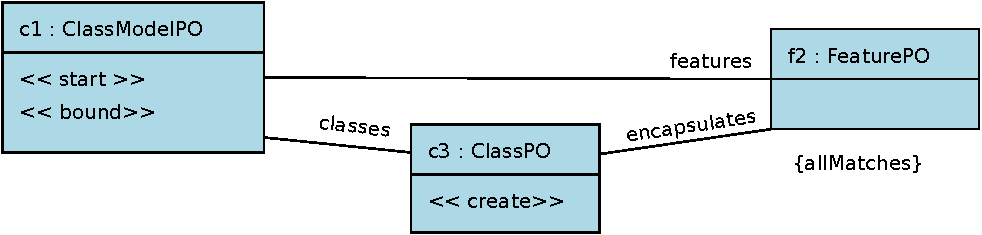
\includegraphics[width=0.8\linewidth]{images/RuleAddInitialClasses.pdf}
 \caption{Rule adding initial classes}
 \label{fig:RuleInitialClasses}
\end{figure}

Figure~\ref{fig:ActivityObjectDiagram} shows an object diagram depicting the activity diagram of test 2 of the model execution case during execution. The \texttt{InitialNode} \texttt{i14} 
and the \texttt{ForkNode} \texttt{f3} have already been added to the \texttt{Trace} 
\texttt{t15}. \texttt{Activity} \texttt{a1} has a \texttt{Token} \texttt{t2} currently
pointing to \texttt{ForkNode} \texttt{f3}. On execution, the \texttt{ForkNode} will remove itself from the set of \texttt{currentElements} of the \texttt{Token} and will add its 
outgoing \texttt{ControlFlow} objects \texttt{c12} and \texttt{c4} to the \texttt{currentElements} instead. In the next turn, one of the control flows (e.g. \texttt{c12}) 
will remove itself from the \texttt{currentElements} and add its target object (e.g. 
\texttt{o11} instead. In addition, the \texttt{noOfVisitors} attribute of the target object 
is incremented. Later on, when the \texttt{JoinNode} \texttt{j7} is executed, 
\texttt{j7} checks its \texttt{noOfVisitors}. If this is lower than the number of 
incoming \texttt{ControlFlow}s, not all parallel executions have reached the \texttt{JoinNode}
yet and thus, the \texttt{JoinNode} deletes the \texttt{currentElements} link but does not 
forward it. Only when \texttt{noOfVisitors} indicates that all parallel branches have reached 
the \texttt{JoinNode}, the \texttt{currentElements} link is forwarded to the \texttt{outgoing}
\texttt{ControlFlow}.  


\begin{figure}[ht] \centering
	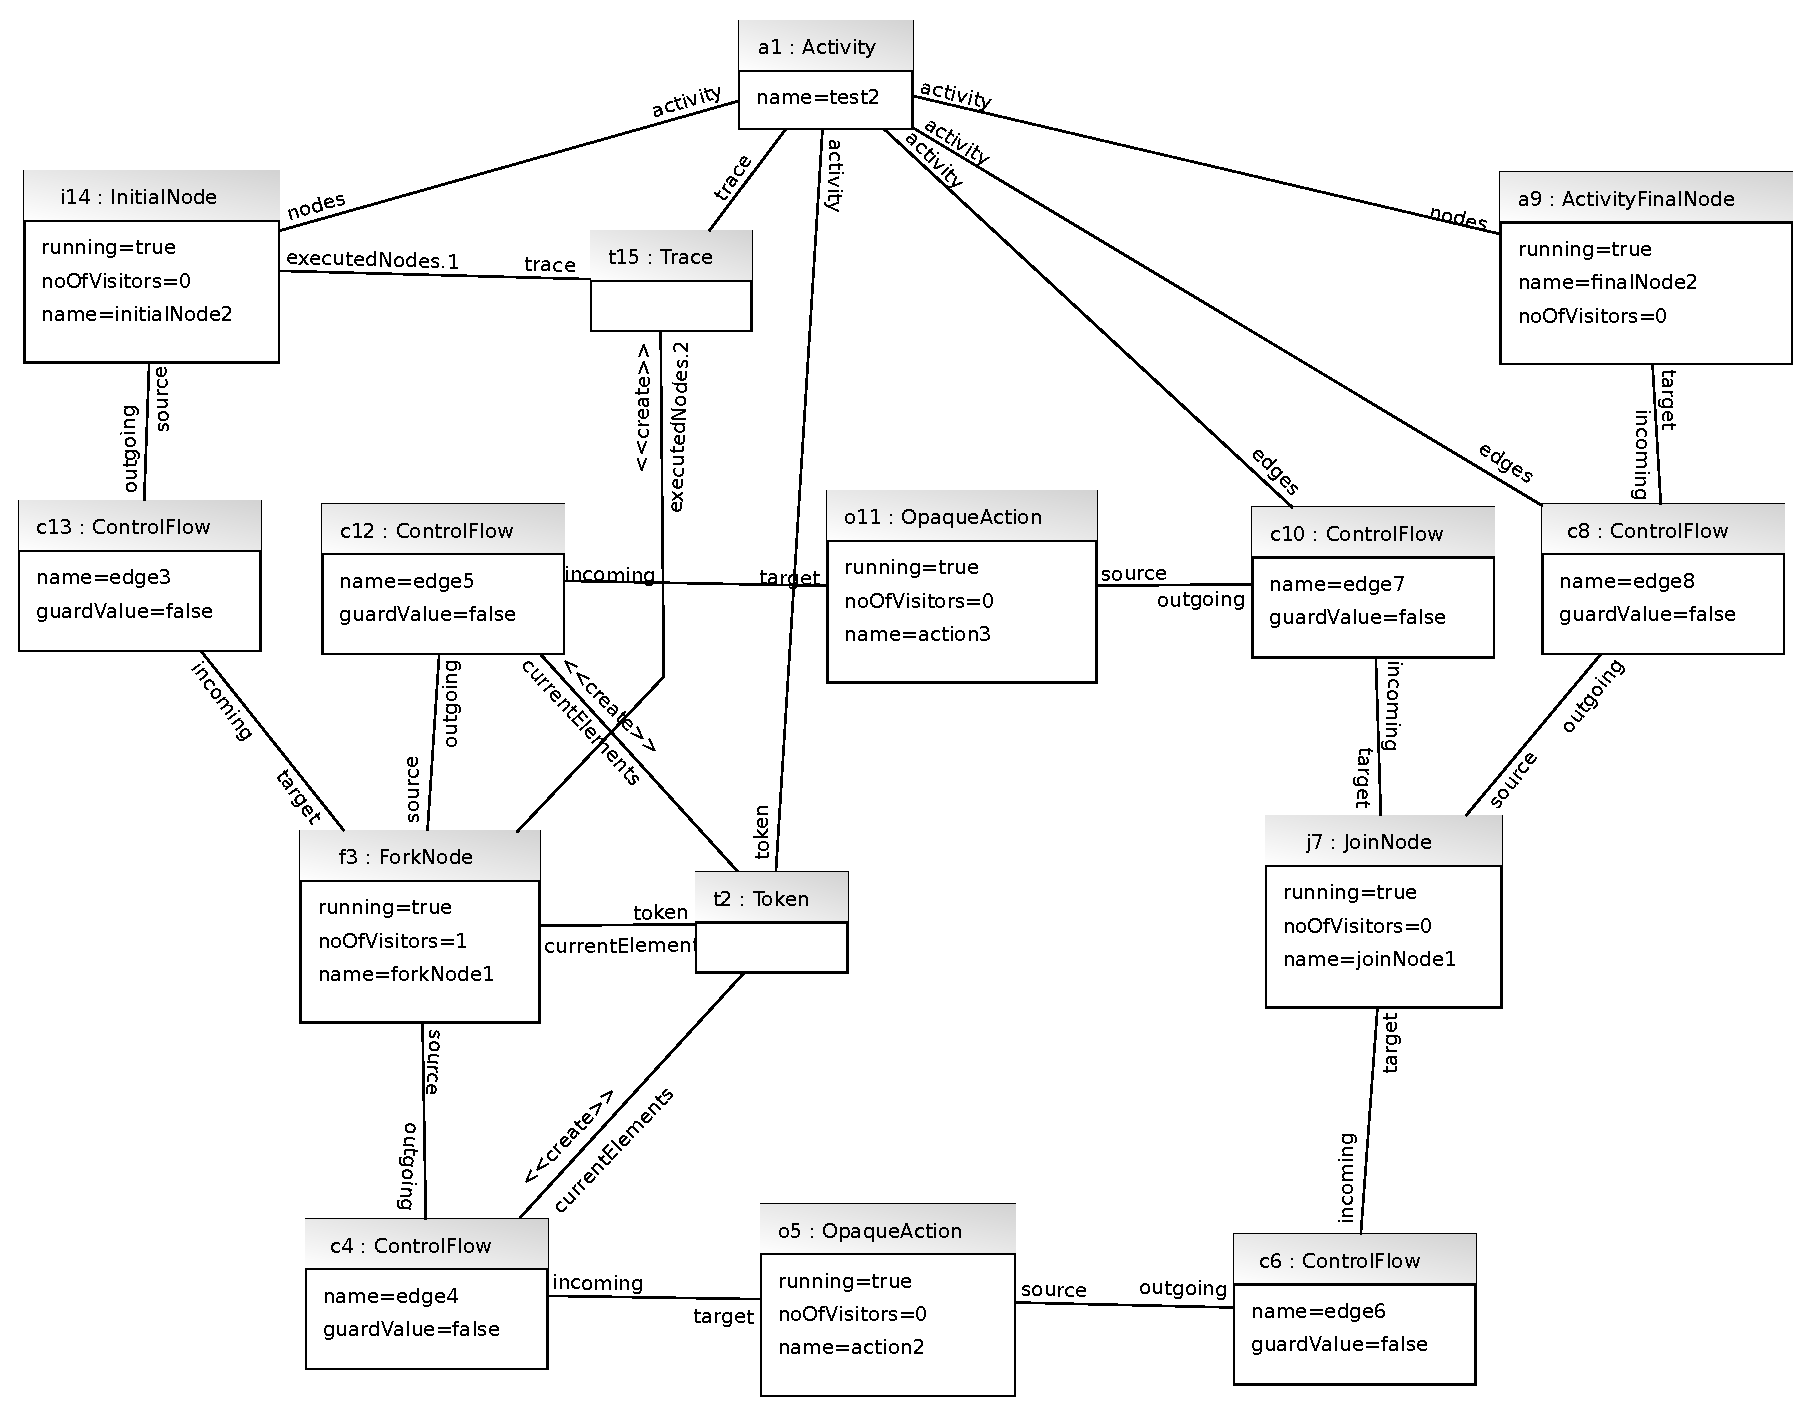
\includegraphics[width=\linewidth]{images/ActivityObjectDiagram.eps}
 \caption{Moving the Token through the Activity Diagram}
 \label{fig:ActivityObjectDiagram}
\end{figure}


\section{The model execution transformations}
\label{sec:ModelExecutionTrafos}

As a start, Listing~\ref{Activity.initVariables.java} shows the Java source code 
that builds and runs the SDMLib model transformation initializing the variables
of an activity. Figure~\ref{fig:Activity.initVariables} shows this transformation 
graphically\footnote{SDMLib is able to render a model transformation as HTML or SVG.}. 


\begin{lstlisting}[language=Java, numbers=left, captionpos=b, 
label=Activity.initVariables.java, escapeinside={\%}{\%},
caption={Initialize variables transformation in Java}
]
class Activity {
    public void initVariables(){
        ActivityPO activityPO = new ActivityPO(this);
        VariablePO localVariablePO = activityPO.hasLocals();
        ValuePO valuePO = localVariablePO.hasInitialValue();
        localVariablePO.createCurrentValue(valuePO);
        localVariablePO.doAllMatches();
    }
\end{lstlisting}

\begin{figure}[ht] \centering
	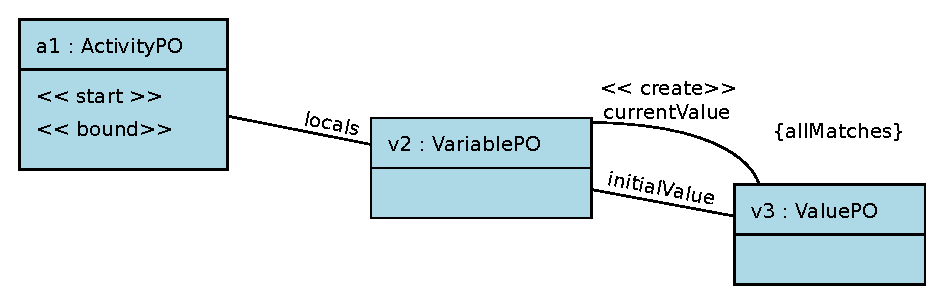
\includegraphics[width=0.8\linewidth]{images/Activity.initVariables.eps}
 \caption{Initialize variables transformation}
 \label{fig:Activity.initVariables}
\end{figure}

In SDMLib a model transformation is called a \emph{Pattern} and it consists 
of \emph{Pattern Objects} and \emph{Pattern Links} that are matched against 
actual model objects. For the initialization of activity variables we use a 
Pattern with three Pattern Objects: \texttt{activityPO}, \texttt{localVariablePO}, 
and \texttt{valuePO}. The constructor call \texttt{new~ActivityPO(this)} creates 
the Pattern and adds the \texttt{activityPO} Pattern Object to it and binds 
\texttt{activityPO} to the current model object \texttt{this}. This means, 
the Pattern Object \texttt{activityPO} is directly matched against the 
model object \texttt{this}. It will also serve as start for the pattern 
matching process. 

Next, the command \texttt{activityPO.hasLocals()} creates the Pattern Object 
\texttt{localVariablePO} and a Pattern Link of type \texttt{locals} that connects 
\texttt{activityPO} and \texttt{localVariablePO}. Then, the pattern matching is 
initiated and SDMLib tries to find model objects of type \texttt{Variable}
that are connected to the current \texttt{Activity} object via a \texttt{locals} link. 
If there are multiple candidates, the candidates are stored for as possible matches. 
One of the candidates is chosen as the current match. 
If there is no match for a given Pattern Object, backtracking is initiated and SDMLib 
tries to chose other candidates for previously visited Pattern Objects and then revisits
the current Pattern Object. If backtracking fails, too, the whole matching fails. 
In the current example case let us assume that there are two variables \texttt{v1} and \texttt{v2}. Thus Pattern Object \texttt{localVariablePO} will be matched e.g. against \texttt{v1} and \texttt{v2} will be stored as alternative candidate. 

SDMLib generates the Method \texttt{hasLocals()} within class \texttt{ActivityPO} from the association \texttt{locals} 
between the classes \texttt{Activity} and \texttt{Variable}. For each association role such a \texttt{has} method is generated in the corresponding \texttt{PO} class. These \texttt{has} methods create a Pattern Link according to the role name and a Pattern Object according 
to the role's target class. 

Line~5 of Listing~\ref{Activity.initVariables.java} extends the search Pattern by an \texttt{valuePO} Pattern Object connected to \texttt{localVariablePO} via an \texttt{initialValue} link. Next, line~6 uses method \texttt{createCurrentValue} to extend our model transformation by an action that creates a \texttt{currentValue} link between the model objects matched by \texttt{localVariablePO} and \texttt{valuePO}. This \texttt{create} action is executed only if the Pattern has a successful match. 

Finally, line~7 calls method \texttt{doAllMatches}. Method \texttt{doAllMatches} triggers 
the backtracking of the Pattern search, i.e. we go back to choices where still alternatives 
are available. In our example, this is the matching of \texttt{localVariablePO} to 
\texttt{var1}. Thus, \texttt{localVariablePO} is now re-matched against \texttt{v2} and the 
remaining pattern matching, i.e. the search for a value and the creation of a 
\texttt{currentValue} link is executed again. Method \texttt{doAllMatches} triggers backtracking until the Pattern search and execution fails. Overall, now all local variables of the current activity are initialized.  


Model transformation \texttt{initVariables} is the first operation called within 
method \texttt{run()} of class \texttt{Activity}, cf. Listing~\ref{Activity.run.java}. 
Similarly, method \texttt{input()} uses an \texttt{doAllMatches} transformation to 
assign input values to variables. Lines 5 and 6 each look-up the set of all 
\texttt{ActivitNode} model objects within the current activity. To implement to-many associations SDMLib generates special set classes for all model classes 
as in this case class \texttt{ActivityNodeSet}. These set classes inherit from a general 
container class and in addition for each method of the model class SDMLib generates a similar method in the corresponding set class. For example the method 
\texttt{withRunning(boolean)} of class \texttt{ActivityNode()} results in a similar method in class \texttt{ActivityNodeSet}. In the set class, the generated method iterates through all contained elements and forwards the method call to each of them. 
Thus, line~5 of Listing~\ref{Activity.run.java} is finally calling method 
\texttt{withRunning(boolean)} on each \texttt{ActivityNode} in the current 
\texttt{Activity}. This sets the state of all activity nodes to running. Similarly, 
line~6 sets the \texttt{noOfVisitors} attribute of all activity nodes to \texttt{0};

\begin{lstlisting}[language=Java, numbers=left, captionpos=b, 
label=Activity.run.java, escapeinside={\%}{\%},
caption={Method Activity.run() in Java}
]
class Activity {
    public void run(){
      this.initVariables();
      this.input(input);
      this.getNodes().withRunning(true);
      this.getNodes().withNoOfVisitors(0);
      
      ActivityPO activityPO = new ActivityPO(this);
      ActivityNodePO activityNodePO = activityPO.hasNodes();
      InitialNodePO initialNodePO = activityNodePO.instanceOf(new InitialNodePO());

      activityPO.createTrace();
      tokenPO = activityPO.createToken();
      tokenPO.createCurrentElements(initialNodePO);
         
      // run the token
      Token token = tokenPO.getCurrentMatch();
      
      while ( ! token.getCurrentElements().isEmpty())
      {
         NamedElement first = token.getCurrentElements().first();
         first.run();
      }
      
      this.getNodes().withRunning(false);
    }
\end{lstlisting}

\begin{figure}[ht] \centering
	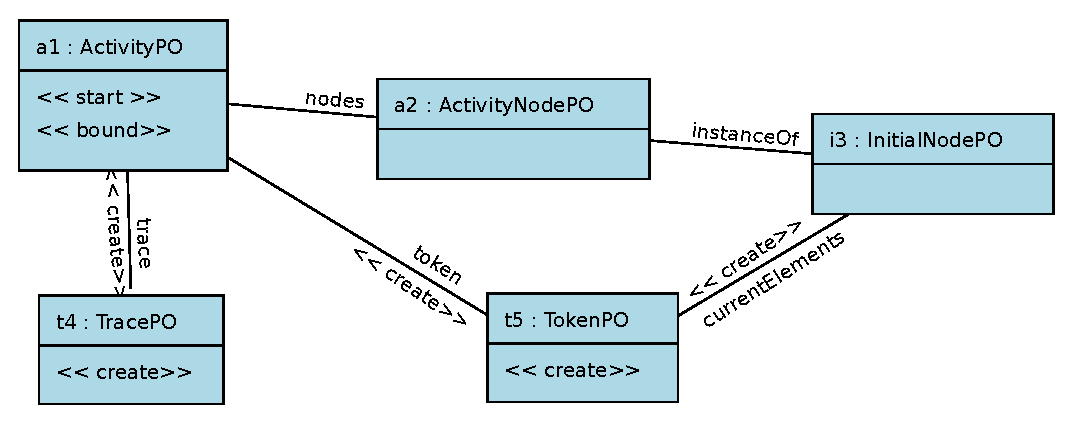
\includegraphics[width=\linewidth]{images/Activity.run.eps}
 \caption{Starting Activity.run() transformation}
 \label{fig:Activity.run}
\end{figure}

Lines 8 to 14 of Listing~\ref{Activity.run.java} build and run the central model 
transformation employed in method \texttt{Activity.run()}. This model transformation 
is shown graphically in Figure~\ref{fig:Activity.run}. Again, the Pattern starts with an \texttt{activityPO} Pattern Object bound to the current \texttt{Activity} model object, 
cf. line~8. This is extended by a \texttt{nodes} link to an \texttt{activityNodePO}, 
cf. line~9. This time we especially look for an activty node of type 
\texttt{InitialNode}. In the current version of SDMLib we have to use a special \texttt{instanceOf()} method to model this type check in our Pattern. This results in another Pattern Object of the desired type in line~10. In the graphical visualization this is rendered by an \texttt{instanceOf} link to another Pattern Object of the 
desired type. However, these two Pattern Object will match against the same model object. As this is somewhat intricate, we plan to enhance SDMLib to generate specific 
\texttt{hasNodesOfTypeInitalNode} methods that include the type check, internally.  

Once we have identified the initial node, we create a \texttt{Trace} object (line~12) 
and a \texttt{Token} object (line~13). Finally, the method call 
\texttt{createCurrentElements(initialNodePO)} creates a \texttt{currentElements} link between the model objects matched by \texttt{tokenPO} and \texttt{initialNodePO} (line~14).

Generally, the described model transformation searches through all nodes of the given activity 
in order to find the node of type \texttt{InitialNode}. This has a runtime complexity of O(n) in the number of activity nodes. However, in the example cases, the initial node is always the first node in the list of activity nodes. Thus, the pattern search always succeeds on the first activity node it visits and thus the actual runtime is O(1).

Once the \texttt{Trace} and the \texttt{Token} object are created, the actual execution 
of the activity diagram is driven by lines 17 through 23 of Listing~\ref{Activity.run.java}. 
First, we look up the model object \texttt{token} that correspond to the Pattern Object 
\texttt{tokenPO} (line~17). The loop of line~19 uses the \texttt{currentElements} link of our 
\texttt{token} object as a queue, it looks-up the first element and calls \texttt{run()} on it. 
The \texttt{run} method will remove the corresponding \texttt{currentElements} link and add 
new (successor) elements to the \texttt{currentElements} instead. Note, \texttt{currentElements}
may point to \texttt{ActivityNode} objects as well as to \texttt{ActivityEdge} objects. 
Thus, loop variable \texttt{first} uses the common super type \texttt{NamedElement}. 

Method \texttt{run()} of class \texttt{NamedElement} is overridden within its subclasses to achieve specific behavior for the various activity diagram elements. 
Listing~\ref{ActivityNode.run.java} and Figure~\ref{fig:ActivityNode.run} show the general behavior of activity nodes.

\begin{lstlisting}[language=Java, numbers=left, captionpos=b, 
label=ActivityNode.run.java, escapeinside={\%}{\%},
caption={Method ActivityNode.run() in Java}
]
class ActivityNode {
    public void run(){
      ActivityNodePO activityNodePO = new ActivityNodePO(this);
         
      // add to trace
      TracePO tracePO = activityNodePO.hasActivity().hasTrace();
      tracePO.createExecutedNodes(activityNodePO);

      // consume token
      TokenPO tokenPO = activityNodePO.hasToken();
      tokenPO.destroyCurrentElements(activityNodePO);
         
      // forward token to all outgoing edges
      ActivityEdgePO activityEdgePO = forkNodePO.hasOutgoing();

      tokenPO.createCurrentElements(activityEdgePO);
         
      activityEdgePO.doAllMatches();
    }
\end{lstlisting}

\begin{figure}[ht] \centering
	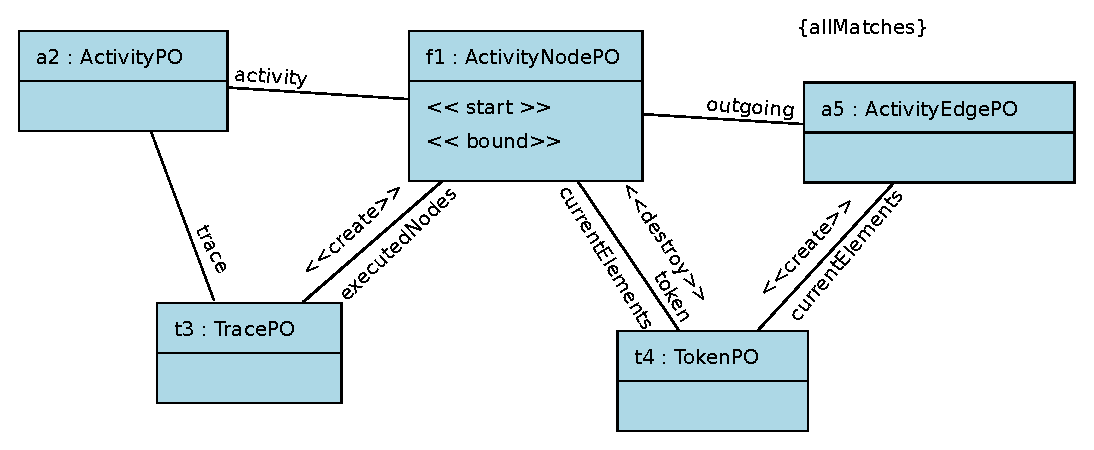
\includegraphics[width=\linewidth]{images/ActivityNode.run.eps}
 \caption{General ActivityNode.run() transformation}
 \label{fig:ActivityNode.run}
\end{figure}

Generally, the model transformation executing an \texttt{ActivityNode} starts 
with an activityNodePO Pattern Object bound to the model object \texttt{this}, cf. line~3 of Listing~\ref{ActivityNode.run.java}. Then, line~6 uses a chain of \texttt{has} operations to look-up the owning \texttt{Activity} and the attached \texttt{tracePO}. Line~7 adds the current \texttt{ActivityNode} to the \texttt{Trace}. Then, we look up the \texttt{tokenPO} that is attched to the current \texttt{ActivityNode} (line~10) and remove the corresponding \texttt{currentElements} link (line~11). Now we forward the token. Thus, line~14 looks for \texttt{outgoing} \texttt{activityEdgePO} matches and line~16 adds such \texttt{ActivityEdge} objects to the current \texttt{Token}. As there may be multiple \texttt{outgoing} \texttt{ActivityEdge} objects, line~18 asks the current Pattern to apply on all matches. Thus all \texttt{outgoing} \texttt{ActivityEdge}s are added to the \texttt{currentElements}. 

Note, the activity diagrams used as test cases provided by case description have no usual activity nodes that have more than one outgoing control flow. Only, fork nodes and decision nodes have multiple outgoing edges. For fork nodes, the general behavior works fine. For decision nodes, we override the 
\texttt{run()} method and extend the general execution pattern by a check for the guard of the 
outgoing \texttt{ActivityEdge}. Only if the guard is true, the corresponding activity edge 
is added to the \texttt{currentElements}. For decision nodes, it is guaranteed, that only one 
outgoing control flow has a guard that evaluates to true. Thus, we do not need an \texttt{allMatches} for decision nodes. For \texttt{JoinNode}s we just extend the general \texttt{ActivityNode.run()} pattern with a check whether the \texttt{noOfVisitors} equals the number of incomming \texttt{ControlFlow}s. Only then the \texttt{Token} is forwarded.  

Listing~\ref{ControlFlow.run.java} and Figure~\ref{fig:ControlFlow.run} show the execution of \texttt{ControlFlow} objects. Line~4 starts with a \texttt{controlFlowPO} Pattern Object bound to the current \texttt{ControlFlow} model object. Line~5 adds the current \texttt{tokenPO}. In any case, we destroy the \texttt{currentElements} link to the \texttt{Token} as the \texttt{ControlFlow} is now executed. Now we want to ensure that the guard of the \texttt{ControlFlow} allows the execution. Actually, this is not necessary as the decision node does not add a \texttt{ControlFlow} to the \texttt{currentElements} unless its guard is true. However, for completeness, \texttt{ControlFlow.run()} checks this condition, too. Unfortunately, there are two different cases to consider: first the \texttt{ControlFlow} may have no guard at all. Then it shall be consider to be true. And second, if the \texttt{ControlFlow} has a guard, than the value of that guard has to be true. To cover both cases at once, we ensure that the \texttt{ControlFlow} has no guard with value false. This may fail if there is no guard or if the guard is true. If it fails, we move the token forward. In our model transformation we use a negative application condition \emph{NAC}, cf. line 11 through 18. The sub pattern within the NAC tries to find a match. If that succeeds, the NAC fails and the overall pattern is not executed, any more. Line~13 and 14 look-up a \texttt{Guard} at the \texttt{controlFlowPO} and test that this \texttt{Guard} is an instance of a \texttt{BooleanVariable} and that this \texttt{BooleanVariable} has a \texttt{currentValue}. Line~16 then ensures that the \texttt{currentValue} is instance of a \texttt{BooleanValue} and that the \texttt{BooleanValue} has the \texttt{value} \texttt{false}. 

\begin{lstlisting}[language=Java, numbers=left, captionpos=b, 
label=ControlFlow.run.java, escapeinside={\%}{\%},
caption={Method ControlFlow.run() in Java}
]
public class ControlFlow extends ActivityEdge{
   @Override
   public void run(){
      ControlFlowPO controlFlowPO = new ControlFlowPO(this);
      TokenPO tokenPO = controlFlowPO.hasToken();

      // in any case remove from currentElements
      tokenPO.destroyCurrentElements(controlFlowPO);

      // add successor if guard allows
      controlFlowPO.startNAC();

      ValuePO valuePO = controlFlowPO.hasGuard()
			   .instanceOf(new BooleanVariablePO()).hasCurrentValue();

      valuePO.instanceOf(new BooleanValuePO()).hasValue(false);

      controlFlowPO.endNAC();

      // OK, move token
      ActivityNodePO targetPO = controlFlowPO.hasTarget();

      tokenPO.createCurrentElements(targetPO);

      // count visits
      targetPO.exec((node) -> node.incrementNoOfVisitors(1));
   }
\end{lstlisting}

\begin{figure}[ht] \centering
	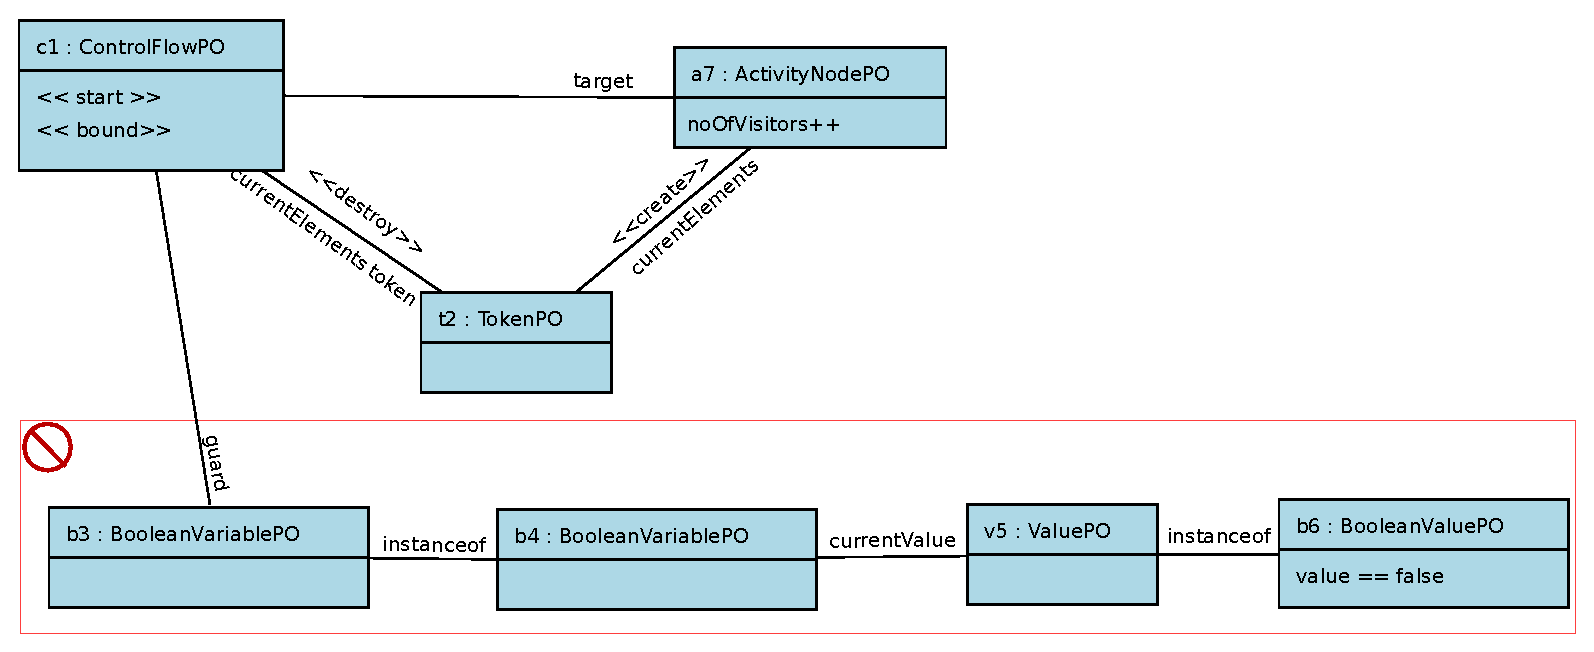
\includegraphics[width=\linewidth]{images/ControlFlow.run.eps}
 \caption{General ActivityNode.run() transformation}
 \label{fig:ControlFlow.run}
\end{figure}

If there is no guard preventing it, line~21 of Listing~\ref{ControlFlow.run.java} identifies the \texttt{target} of our \texttt{ControlFlow} and line~23 adds this target to the \texttt{currentElements}. Finally, line~26 uses a lambda expression to add an operation to our model transformation that on execution increments the \texttt{noOfVisitors} of the \texttt{target}. 

\texttt{OpaqueAction} nodes may have a number of \texttt{expressions} attached to them. \texttt{Expression} objects provide their own \texttt{run()} methods executing them. Thus, for \texttt{OpaqueAction} nodes we override the \texttt{ActivityNode} \texttt{run()} method to call the \texttt{Expression.run()} method on each expression. The expressions use various subclasses and various enumeration types to distinguish between different operations. Thus, each subclass provides its specific \texttt{run()} method and these specific \texttt{run()} methods use traditional switch statements to deal with the corresponding enumeration types, cf. Listing~\ref{IntegerCalculationExpression.run.java}. Alternatively, we might have provided Model Patterns for each case, however evaluating expression trees is not really the application domain for model patterns. 

\begin{lstlisting}[language=Java, numbers=left, captionpos=b, 
label=IntegerCalculationExpression.run.java, escapeinside={\%}{\%},
caption={Method IntegerCalculationExpression.run() in Java}
]
public class IntegerCalculationExpression extends IntegerExpression
{
   @Override
   public void run()
   {
      IntegerValue val1 = (IntegerValue) this.getOperand1().getCurrentValue();
      IntegerValue val2 = (IntegerValue) this.getOperand2().getCurrentValue();
      int op1 = val1.getValue();
      int op2 = val2.getValue();
      
      int result = 0;
      
      switch (this.getOperator())
      {
      case ADD:
         result = op1 + op2;
         break;

      case SUBRACT:
         result = op1 + op2;
         break;

      default:
         throw new UnsupportedOperationException(""+this.getOperator());
      }
      
      this.getAssignee().setCurrentValue(new IntegerValue().withValue(result));      
   }
\end{lstlisting}



\section{Results}
\label{sec:results}

Once we decided to come up with our own concept for moving tokens, it was pretty straight 
forward to develop the corresponding model transformations. The simplified token concept also resulted in model transformations that do very little search through to-many associations. The model transformations mainly look-up the current situation and and check all kinds of conditions on it. Thus, we think the execution is reasonably fast. The following table shows our performance measurements executed on a laptop with a 64 Bit Intel Dual Core i7 CPU M620 2.67GHz with 8~GB memory.   

\begin{center}
	\begin{tabular} { r c c c c } 
		performance test               & variant 1 & variant 2 & variant 3.1 & variant 3.2 \\
		execution time (milli seconds) & 9.99 ms & 9.25 ms & 9.38 ms & 14.05 ms
	\end{tabular}
\end{center}

For the performance measurement we did the usual tricks like warming up the Java virtual machine hot compiler by executing each activity 1000 times before measurement. We than ran each test 5 times and computed the average runtime. Overall, we think the performance test cases are a little bit to small to measure the model transformation execution time without side effects and overheads from other things running in the virtual machine.  


\section{Summar}
\label{sec:summary}

Overall, the model execution case fits very well to SDMLib. It was quite straight forward to 
model the different execution steps and the different steps have a complexity that justifies the usage of model transformation in comparison to hand written Java code. The class model provided with the case uses a lot of inheritance and enumeration types. Actually, SDMLib can still be improved in dealing with inheritance. This is current work. Enumerations are used e.g. for the operators in expression trees. We evaluate such expression trees with usual Java code. Model transformation seem not to give leverage here. 

\bibliographystyle{abbrv}
\bibliography{fujaba}  

\end{document}

 